\section{Messwerte}
\label{sec:Messwerte}

\begin{table}
    \centering
    \caption{Die Tabelle mit allen vor Ort aufgenommenen Messdaten.}
    \label{tab:DatenAbgelesen}
    \begin{tabular}{
        S[table-format=2.4]
        S[table-format=1.2]
        S[table-format=1.1]
        S[table-format=3]
        S[table-format=4.1]
      }
        \toprule
        {$f \mathbin{/} \unit{\kilo\hertz}$} &
        {$U_c \mathbin{/} \unit{\volt}$} &
        {$U_G \mathbin{/} \unit{\volt}$} &
        {$a \mathbin{/} \unit{\micro\second}$} &
        {$b \mathbin{/} \unit{\micro\second}$} \\
        \midrule
        0.110  & 7.5  & 3.5 & 400 & 4000 \\
        0.189  & 6    & 3.5 & 300 & 2200 \\
        0.250  & 5    & 3.5 & 300 & 1700 \\
        0.2995 & 4    & 3.5 & 250 & 1400 \\
        0.4008 & 3.4  & 3.6 & 200 & 1000 \\
        0.514  & 2.2  & 3.6 & 160 & 840  \\
        0.998  & 1.6  & 3.6 & 100 & 440  \\
        2.051  & 0.8  & 3.6 & 40  & 200  \\
        3.12   & 0.6  & 3.6 & 40  & 140  \\
        5.17   & 0.25 & 3.6 & 20  & 80   \\
        9.08   & 0.2  & 3.6 & 4   & 16   \\
        22.34  & 0.08 & 3.6 & 4   & 20   \\
        30.37  & 0.06 & 3.6 & 4   & 14   \\
        35.15  & 0.05 & 3.6 & 4   & 12   \\
        40.09  & 0.04 & 3.6 & 4   & 12   \\
        42.33  & 0.04 & 3.6 & 2   & 10   \\
        44.05  & 0.04 & 3.6 & 2   & 10   \\
        46.16  & 0.04 & 3.6 & 2   & 10   \\
        48.32  & 0.04 & 3.6 & 2   & 10   \\
        51.24  & 0.03 & 3.6 & 2   & 8.5  \\
        \bottomrule
    \end{tabular}
\end{table}

\begin{figure}
  \centering
  \label{abb:Entladung}
  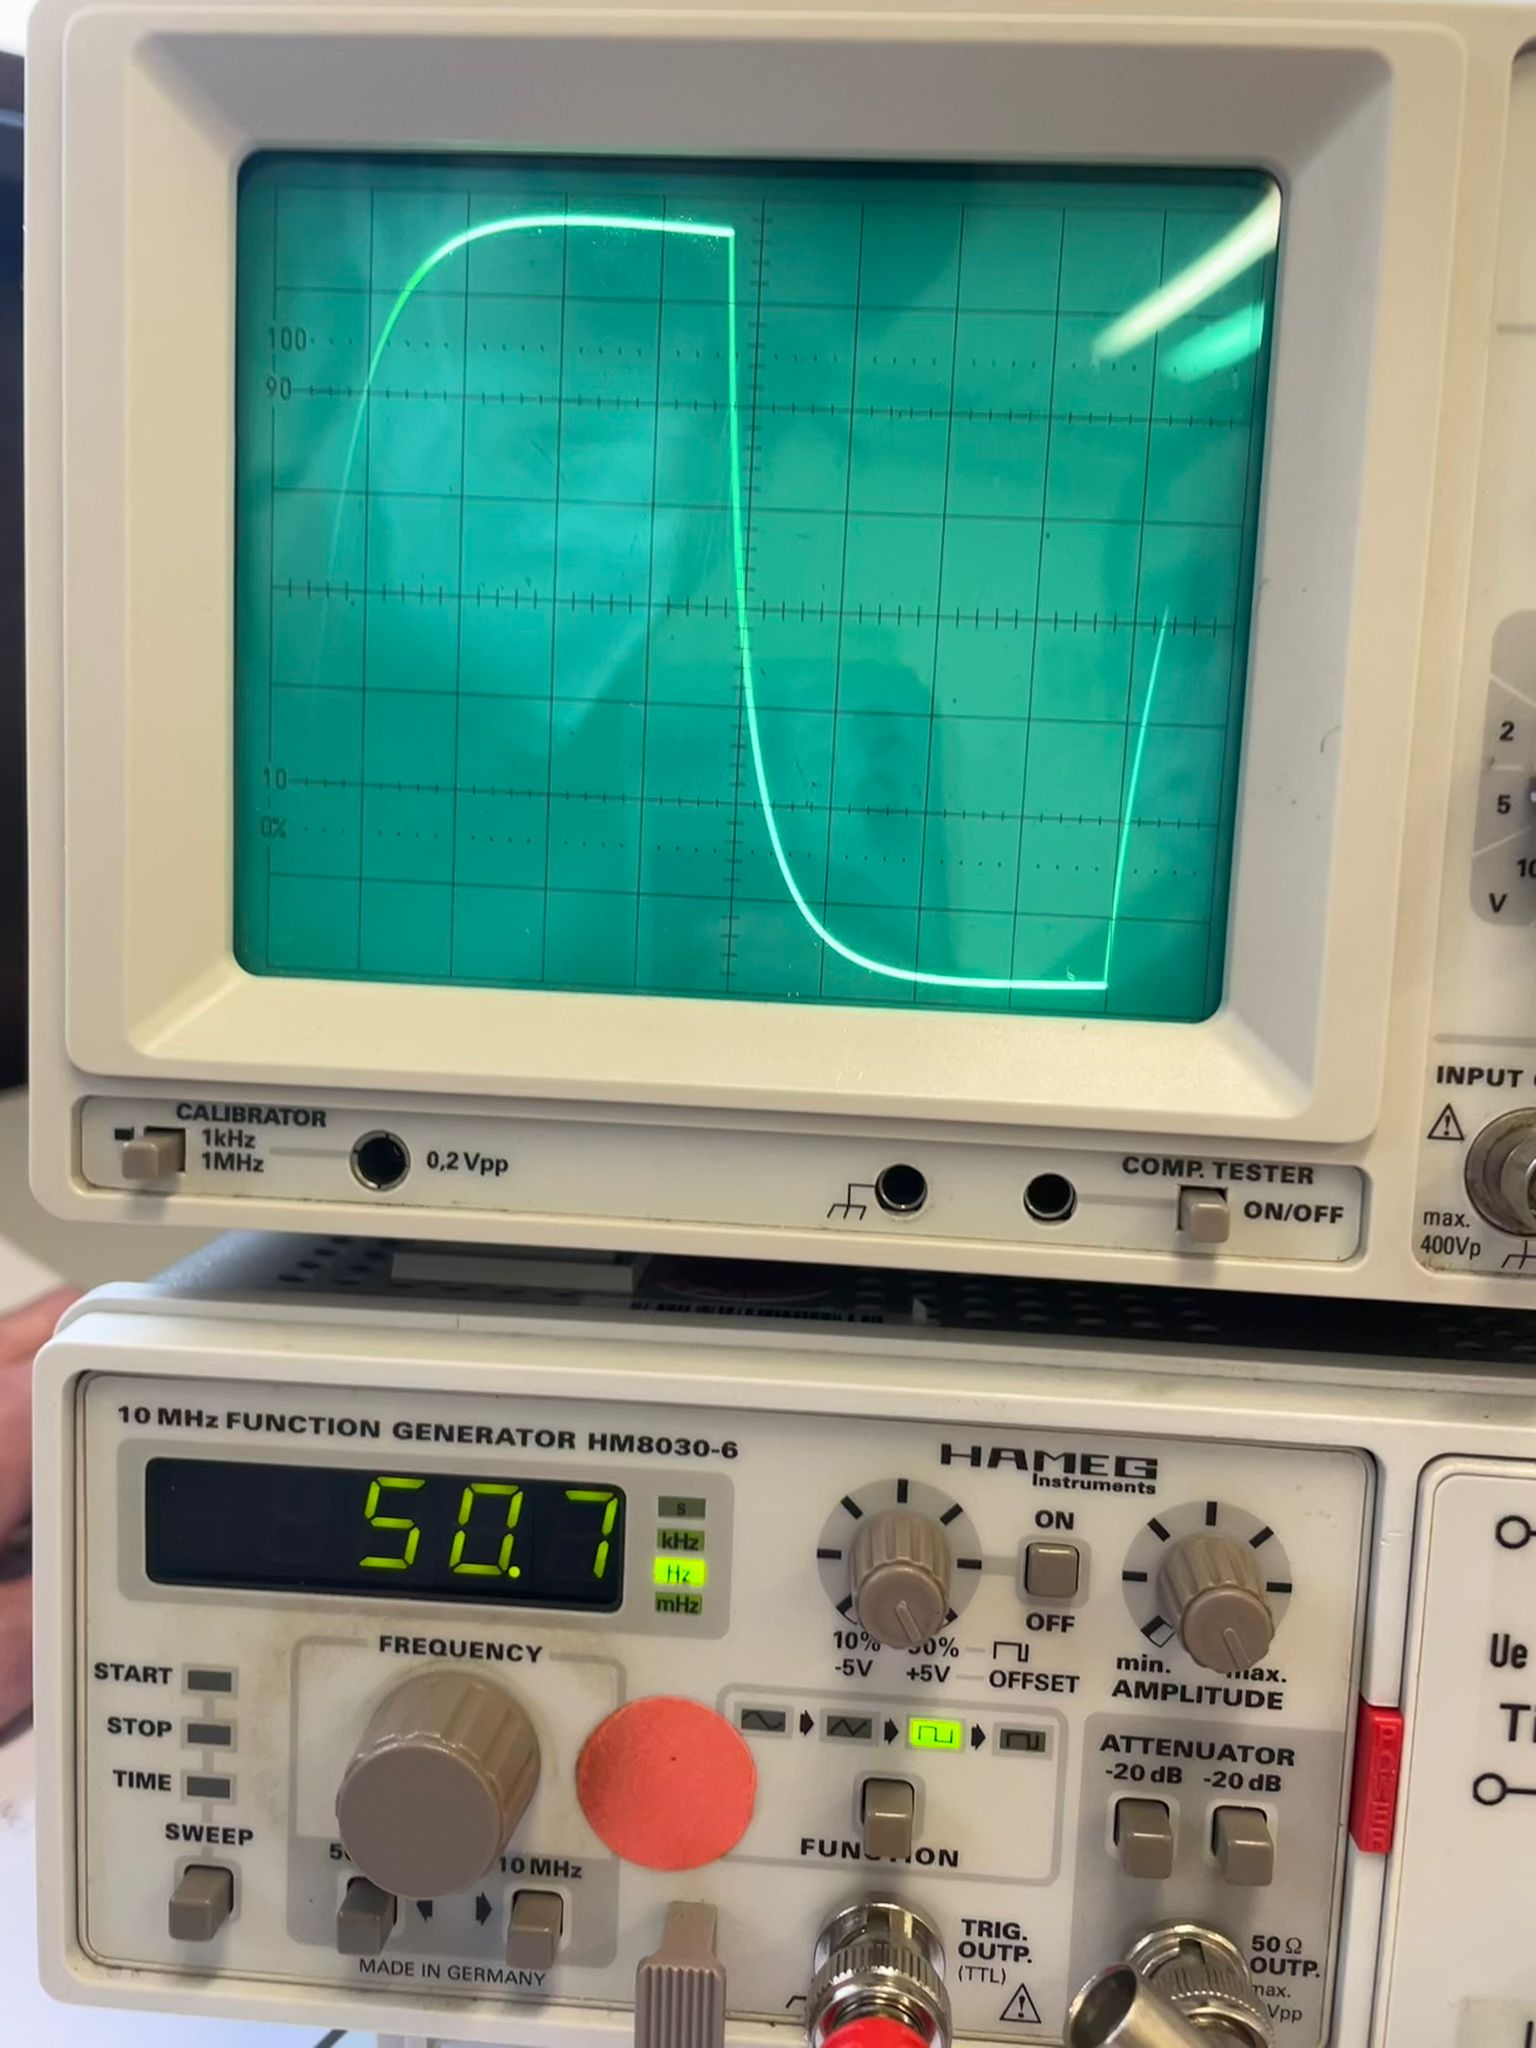
\includegraphics[scale=0.1]{content/entladung.png}
  \caption{Der Entladungsprozess des Kondensators.}
\end{figure}

\begin{table}
    \centering
    \caption{Eine Tabelle mit den aufgenommenen Messdaten aus \autoref{abb:Entladung} des Entladungsprozesses des Kondensators.}
    \label{tab:DatenEntladung}
    \begin{tabular}{
        S[table-format=1.1]
        S[table-format=1.2]
        S[table-format=-1.3]
        @{\hspace*{3em}\hspace*{\tabcolsep}}
        S[table-format=1.1]
        S[table-format=1.2]
        S[table-format=-1.3]
      }
        \toprule
        {$U_c \mathbin{/} \unit{\volt}$} &
        {$t \mathbin{/} \unit{\milli\second}$} &
        {$\ln(\frac{U_c}{U_0})$} &
        {$U_c \mathbin{/} \unit{\volt}$} &
        {$t \mathbin{/} \unit{\milli\second}$} &
        {$\ln(\frac{U_c}{U_0})$} \\
        \midrule
        3.4 & 0.04 & -0.057 & 1.6 & 0.3  & -0.811 \\
        3.2 & 0.08 & -0.118 & 1.4 & 0.34 & -0.944 \\
        3   & 0.09 & -0.182 & 1.2 & 0.48 & -1.099 \\
        2.8 & 0.1  & -0.251 & 1   & 0.53 & -1.281 \\
        2.6 & 0.13 & -0.325 & 0.8 & 0.62 & -1.504 \\
        2.4 & 0.16 & -0.405 & 0.6 & 0.73 & -1.792 \\
        2.2 & 0.19 & -0.492 & 0.4 & 0.9  & -2.197 \\
        2   & 0.24 & -0.588 & 0.2 & 1.1  & -2.890 \\
        1.8 & 0.28 & -0.693 & 0.1 & 1.4  & -3.584 \\
        \bottomrule
    \end{tabular}
\end{table}

\begin{table}
    \centering
    \caption{Eine Tabelle mit den Wertepaaren für Aufgabenteil b)}
    \label{tab:DatenB}
    \begin{tabular}{
        S[table-format=2.4]
        S[table-format=1.2]
      }
        \toprule
        {$f \mathbin{/} \unit{\kilo\hertz}$} &
        {$\frac{U_c}{U_0} \mathbin{/} \unit{\volt}$} \\
        \midrule
        0.110  & 2.083 \\
        0.189  & 1.667 \\
        0.250  & 1.389 \\
        0.2995 & 1.111 \\
        0.4008 & 0.944 \\
        0.514  & 0.611 \\
        0.998  & 0.444 \\
        2.051  & 0.222 \\
        3.12   & 0.167 \\
        5.17   & 0.069 \\
        9.08   & 0.056 \\
        22.34  & 0.022 \\
        30.37  & 0.017 \\
        35.15  & 0.014 \\
        40.09  & 0.011 \\
        42.33  & 0.011 \\
        44.05  & 0.011 \\
        46.16  & 0.011 \\
        48.32  & 0.011 \\
        51.24  & 0.008 \\
        \bottomrule
    \end{tabular}
\end{table}

\begin{table}
    \centering
    \caption{Eine Tabelle mit den Wertepaaren für Teilaufgabe c) mit den aus den Messwerten von a und b aus \autoref{tab:DatenAbgelesen} mit Formel (??) berechneten $\varphi$.}
    \label{tab:DatenC}
    \begin{tabular}{
        S[table-format=2.4]
        S[table-format=1.4]
      }
        \toprule
        {$f \mathbin{/} \unit{\kilo\hertz}$} &
        {$\symup{\varphi} \mathbin{/} \unit{\radian}$}\\
        \midrule
        0.110  & 0.6283 \\
        0.189  & 0.8568 \\
        0.250  & 1.1088 \\
        0.2995 &  1.122 \\
        0.4008 & 1.2566 \\
        0.514  & 1.1968 \\
        0.998  &  1.428 \\
        2.051  & 1.2566 \\
        3.12   & 1.7952 \\
        5.17   & 1.5708 \\
        9.08   & 1.5708 \\
        22.34  & 1.2566 \\
        30.37  & 1.7952 \\
        35.15  & 2.0944 \\
        40.09  & 2.0944 \\
        42.33  & 1.2566 \\
        44.05  & 1.2566 \\
        46.16  & 1.2566 \\
        48.32  & 1.2566 \\
        51.24  & 1.4784 \\
        \bottomrule
    \end{tabular}
\end{table}

\begin{table}
  \centering
  \caption{Die Wertepaare für den Polarplot}
  \label{tab:DatenD}
  \begin{tabular}{
      S[table-format=1.3]
      S[table-format=1.4]
    }
      \toprule
      {$\frac{U_c}{U_0} \mathbin{/} \unit{\volt}$} &
      {$\symup{\varphi} \mathbin{/} \unit{\radian}$}\\
      \midrule
      2.083 & 0.6283 \\
      1.667 & 0.8568 \\
      1.389 & 1.1088 \\
      1.111 &  1.122 \\
      0.944 & 1.2566 \\
      0.611 & 1.1968 \\
      0.444 &  1.428 \\
      0.222 & 1.2566 \\
      0.167 & 1.7952 \\
      0.069 & 1.5708 \\
      0.056 & 1.5708 \\
      0.022 & 1.2566 \\
      0.017 & 1.7952 \\
      0.014 & 2.0944 \\
      0.011 & 2.0944 \\
      0.011 & 1.2566 \\
      0.011 & 1.2566 \\
      0.011 & 1.2566 \\
      0.011 & 1.2566 \\
      0.008 & 1.4784 \\
      \bottomrule
  \end{tabular}
\end{table}